
\chapter{Experiments}

In this chapter, the experimental setup used in this project is detailed.
\section{Tools used}

\subsection{Hardware}
Deep learning models were trained on a machine with Intel i7-6800K hexacore CPU with an NVIDIA GPU GTX 1080 GPU. Development was done on the author's personal laptop, a 2014 MacBook Pro with Intel i5 Core.

\subsection{Language and environment}
R and Python were candidates considered for development. Python 3.5 was used for the project as Python is more efficient when handling large datasets, and better compared to R from a deployment perspective.
Initially, Jupyter Notebooks were used for exploration and development. However, Jupyter proved to be inefficient while deploying code, the code was written and run in Python files developed in a basic code editor, Sublime Text\cite{noauthor_sublime_nodate}. 

\subsection{Deep Learning Framework}
There are many libraries available for implementing neural networks. The most common among them are TensorFlow\cite{noauthor_TensorFlow:_2018}, Keras\cite{noauthor_keras_nodate}, PyTorch\cite{noauthor_pytorch_nodate}, CNTK\cite{noauthor_microsoft_2018}, MXNet\cite{noauthor_incubator-mxnet:_2018}. Due to its heavy popularity in tutorials, Keras and TensorFlow were the major choice to be made. Keras is a high-level abstraction, and can be used in combination with either of TensorFlow or Pytorch. Keras is easy to learn for a beginner, and well documented, with many standard networks to be easily implemented with a few lines of code. However, TensorFlow was chosen for this work with the notion that there might be the need to build networks that are much complicated. For more complicated implementations, Keras does not have straightforward solutions, and TensorFlow is recommended. 
Finally, TensorFlow version 1.9 for GPU was employed in this work.

Additional requirements for the smooth working of TensorFlow for GPU, mentioned in the official TensorFlow documentation age, CUDA and CuDNN. CUDA version 9.0 and CuDNN version 7.0 were installed on the systems.



\subsection{Version control and Tracking}
In order to keep track of progress and efficeintly store several versions, git was used . In order to facilitate transition between the 2 machines that were used, Github was used. All the code developed in this project is present in \url{https://github.com/pattern-recogniser/pedestrian-trajectory-predictor}

\section{Dataset}
From the previous chapter, it is evident that there is heavy research being done for trajectory prediction in the domain of crowd forecasting, and subsequently the majority of data sources come from crowd surveillance. 
Several trajectory datasets were considered. However, as it would be best to use a source that would give the most data, it was decided to use the dataset from Socially Aware Crowd Forecasting. 
An interesting point to be noted is that in the case of pedestrian trajectory prediction in a traffic setting, there are no benchmark datasets.
\begin{table}[h]
\begin{tabular}{|l|l|l|}
\hline
Dataset     & Domain            & \# of pedestrians \\
\hline
ETH**       & Crowd forecasting      & 360          \\
\hline
UCY*        & Crowd forecasting      & 204          \\
\hline
Zara-01*    & Crowd forecasting      & 204          \\
\hline
Zara-02*    & Crowd forecasting      & 207          \\
\hline
Social-LSTM & Crowd forecasting      & 14k          \\
\hline
Poly-MLP    & Pedestrian \& Cyclists & 1068 pedestrian, 464 cyclist trajectories\\
\hline
\end{tabular}
\caption{Datasets considered}
\label{table:dataset_considered}

\end{table}

\subsection{Data Understanding}

The dataset used is a set of trajectories collected from a train station from the work of Alahi et al.\cite{alahi_socially-aware_2014}. It consists of 42 million trajectories. 
The data is split across 13 files that are in .csv format, with each file having around 4 million rows each. Each file represents one day's recorded data. The data is sampled at 100 millisecond intervals. Each row in the .csv file is a combination of time-stamp, x-coordinate and y-coordinate position in millimetres from the origin, which is the top left of the image. There are on average 1000 pedestrians in each file. The total size of the file amounts to 6 GB of data.
\begin{figure}[h]
    \centering
    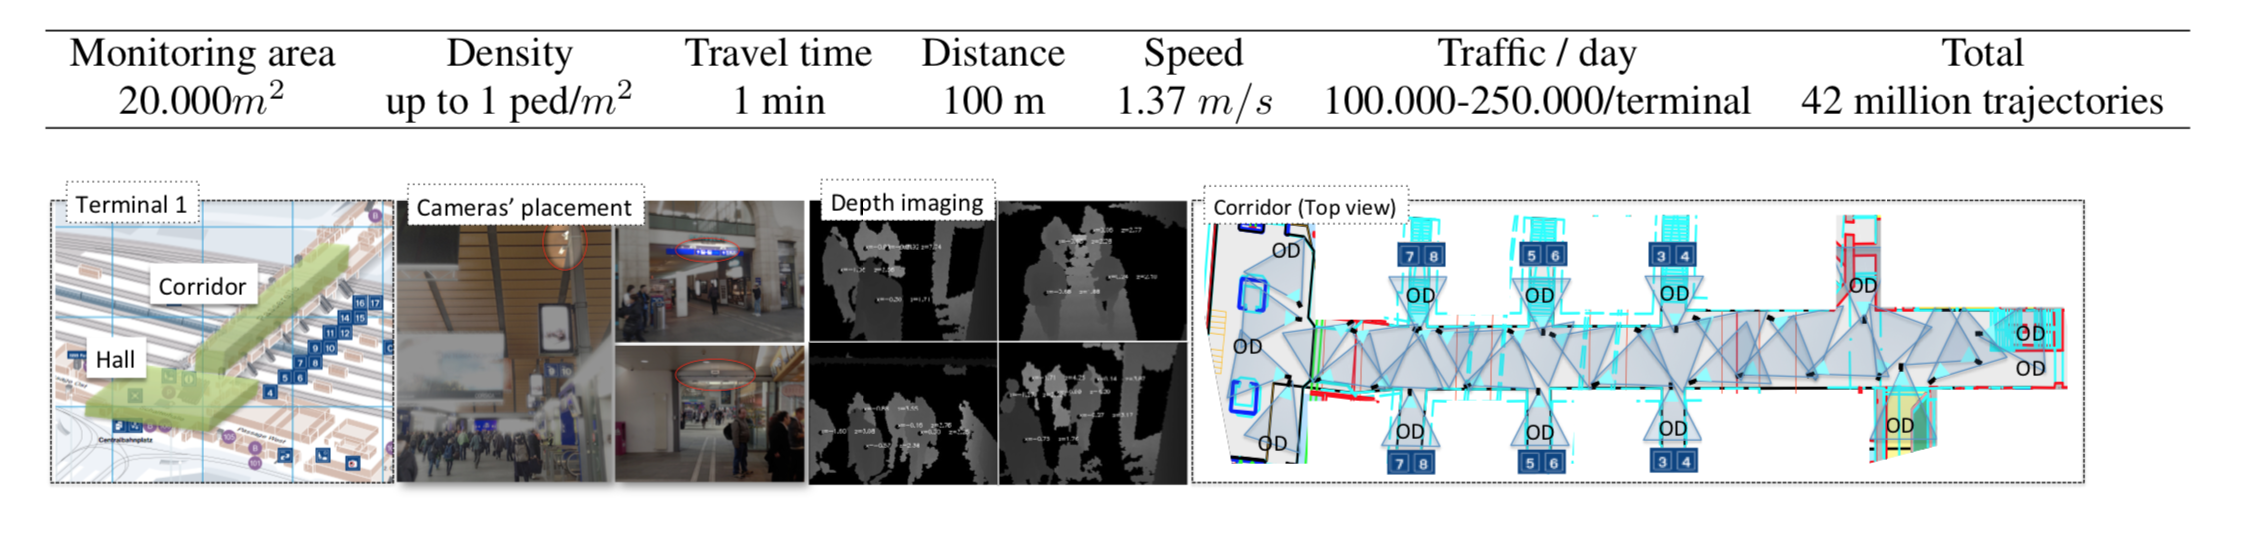
\includegraphics[width=\textwidth]{Figures/Dataset_explanation.png}
    \caption[Key info of Dataset used]{Real-world setup. Top row presents some facts regarding the dataset (values are in average). Bottom row illustrates one of the monitored corridors. More than 30 cameras are deployed in the presented corridor, whereas 132 cameras are deployed in total in 3 corridors, one track, and one large hall. At any given time, the occupancy of the corridor can reach more than one thousand of pedestrians. The label 'OD' represents entry/exit zones \cite{alahi_socially-aware_2014}}

    \label{fig:dataset_explanation}
\end{figure}






\subsection{Data Processing}
\subsubsection{Identifying trajectories}

Each continuous distinct path taken by a pedestrian is identified as a trajectory. Two consecutive positions of the same pedestrian, if observed after a span of 2 seconds are considered belonging to different trajectories.
As the average time difference between consecutive recorded positions of a pedestrian is 100 milliseconds, a threshold of 2 seconds is a conservative one.
Consecutive x or y co-ordinate positions differing by more than 500 millimetres are considered belonging to different trajectories. This is equivalent to clamping the speed of a walking person to \(5 m/s\).
    
\subsubsection{Normalisation of inputs}
In order to speed up the learning algorithm, the input positions have been normalised. The resultant normalised dataset is centred around 0, and has a standard deviation of 1. The minmaxscaler method from sklearn was used to perform normalisation \cite{noauthor_sklearn.preprocessing.minmaxscaler_nodate}.

\subsubsection{Splitting the data}

Data is split into train:test:dev set using a 98:1:1 split. This has been used instead of a standard 70:20:10, as in this case, the data is pretty big, and 1\% of the data would be close to half a million rows. Dev set is another name used for the validation set. Hyper-parameter tuning of the network is done based on performance on the Dev set. Final reported metrics are from the test set. This is to ensure that the performance metric is not specific to the data that we have used for the model, and gives a better measure of the model's performance when it is used for previously unseen data. Results of loss from the dev set are also reported in this document. However, as a performance metric, only the test set metric is used.

\section{Implementation}
\subsection{Data Handling}

As each individual file is big, keeping all the files as a list resulted in Memory error. In order to deal with this, only one file is stored in memory at a time. Each file is read from disk, processed, and finally converted into input format-ready, and then pickled back to disk. When handing data into the network, the data is read from the pickled file on disk, and passed to the network.

\subsection{Network Architecture}
There is one input layer, one hidden layer with 200 RNN units in it, and one output layer. A learning rate of 0.05 was used. Data was fed into the model in a batch of 128. Adam optimiser is used to find the optimal values of parameters.

The observation window considered here is for 1 seconds, and the prediction window is 3 seconds. This has been used keeping in mind that at average driving speeds, the maximum observation time would be 1 second, and predicting 3 seconds ahead will be beneficial for the driver alert mechanism.
\begin{figure}[ht]
    \centering
    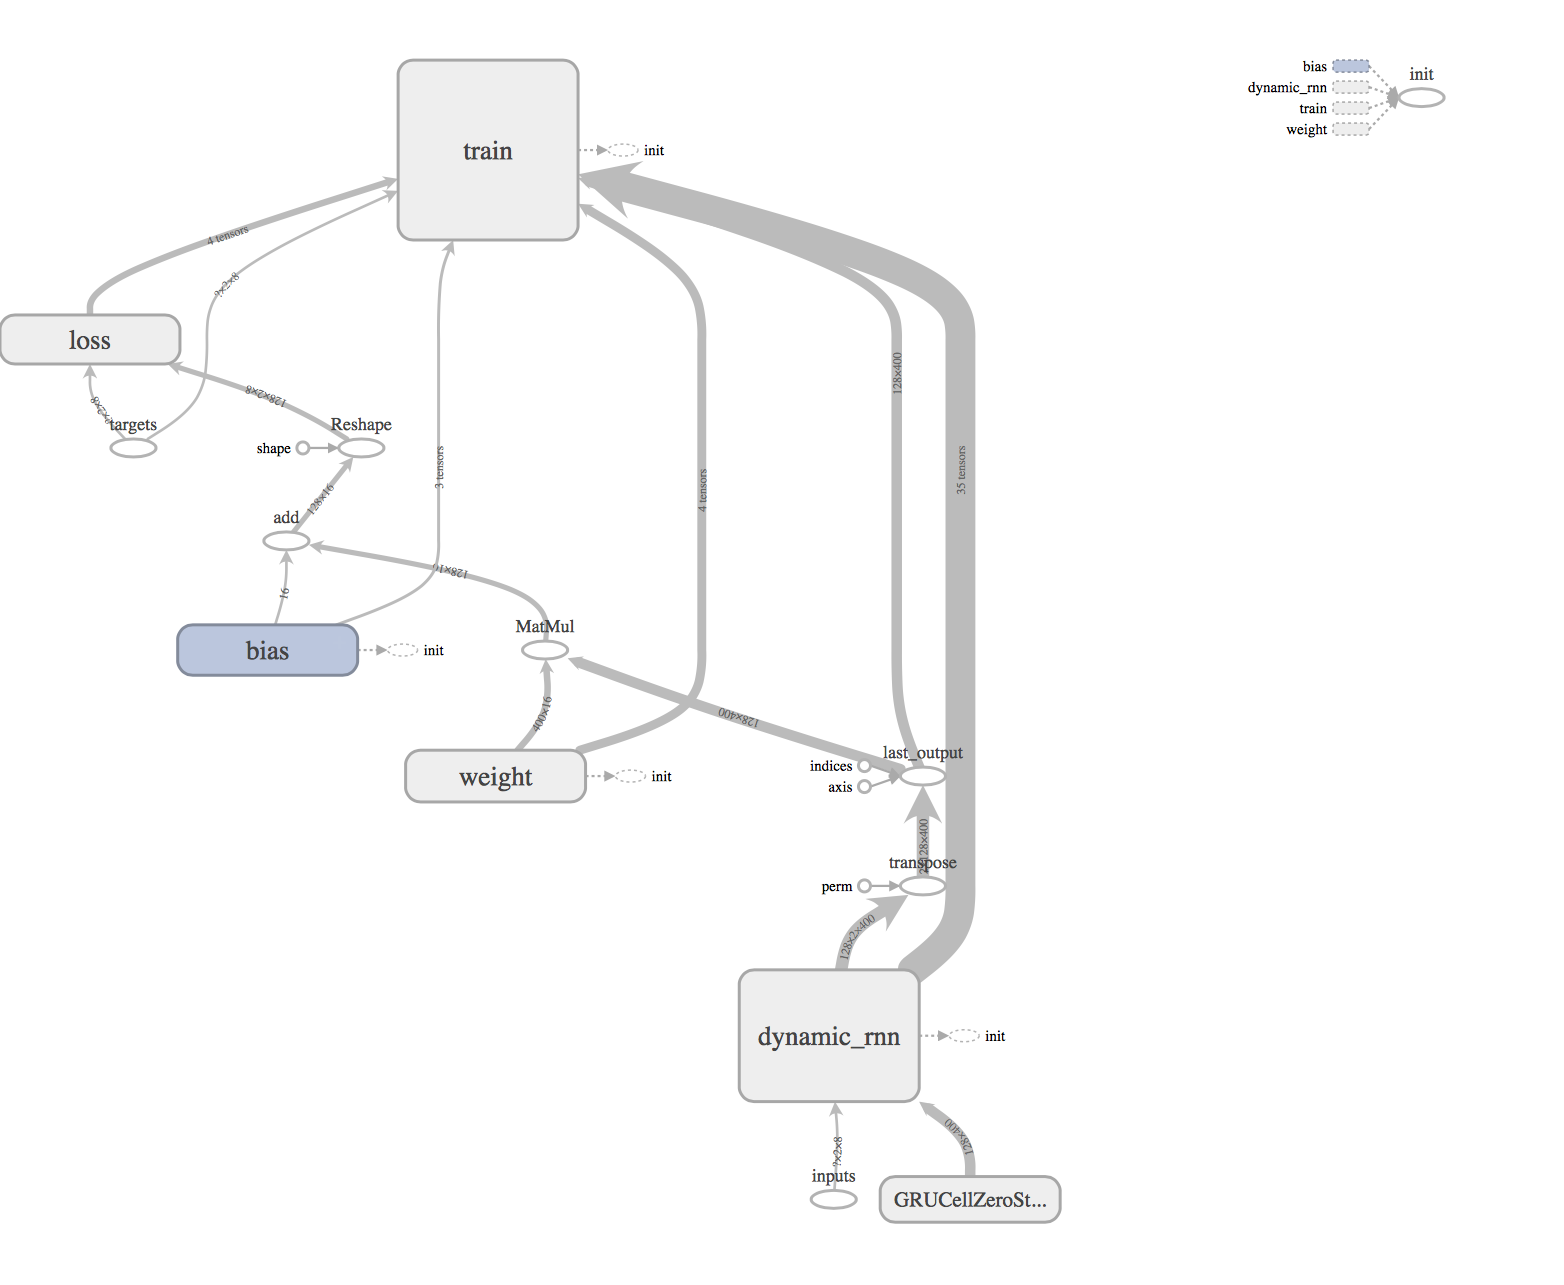
\includegraphics[width=\textwidth]{Figures/TF_graph.png}
    \caption[Network computation]{ Computation graph visualised using TensorBoard}

    \label{fig:tf_graph}
\end{figure}

Figure \ref{fig:tf_graph} represents the TensorFlow graph for computation of the model. In the top right, is the initialisation of the weights, biases in the model.

Loss is the sum of squared Euclidean errors. The hidden state of the GRU is saved and used for prediction. 